
\documentclass{beamer}

\mode<presentation> {

\usetheme{Madrid}

}

\usepackage{graphicx} 
\usepackage{booktabs} 
\usepackage[italian]{babel}
%----------------------------------------------------------------------------------------
%	TITLE PAGE
%----------------------------------------------------------------------------------------

\title[Relazione progetto finale]{Sistema cloud based per la gestione real-time di eventi geolocalizzati}

\author{Francesco Di Franco} % Your name
\institute[UniCT] 
{
Univerist\`a degli studi di Catania \\ % Your institution for the title page
\medskip
\textit{} 
}
\date{09-03-2016} 

\begin{document}
%SLIDE 1
\begin{frame}
\begin{table}[]
\centering
\begin{tabular}{ll}

\begin{minipage}{0.4\textwidth}
\begin{center}

\includegraphics[scale=0.15]{../img/logo_unict.png}
\end{center}
\end{minipage}

&  
\begin{minipage}{0.5\textwidth}


\includegraphics[scale=0.07]{../img/logoPSM.png}

\end{minipage}

\end{tabular}
\end{table}
\titlepage
\end{frame}


%SLIDE 2
\begin{frame}
\frametitle{Park Smart}
Parksmart 
\begin{itemize}
\item Software di videoanalisi
\item Sistema software per la gestione real-time di eventi
\item Applicazione per smartphone
\end{itemize}
\end{frame}

%SLIDE 3

\begin{frame}
\frametitle{Amazon web services}
\begin{columns}[c] 

\column{.45\textwidth} 

\begin{enumerate}
\item ElasticBeanstalk
\item ElasticCache
\item Cognito
\item DynamoDB
\end{enumerate}

\column{.5\textwidth} 
Per lo sviluppo di questo progetto sono state usate le tecnologie cloud di Amazon web services. Grazie ai servizi SaaS usati \`e stato risolto il problema della scalabilit\`a orizzontale delle risorse.

\end{columns}
\end{frame}


%SLIDE 4

\begin{frame}
\frametitle{Componenti sistema real time}
\begin{block}{NodeJs}
Un framework Javascript a eventi che estende l'architettura REST (Http). 
\end{block}

\begin{block}{DynamoDb}
Tecnologia di DBMS NoSql propietaria Amazon.
\end{block}

\begin{block}{Socket.io}
Libreria molto flessibile che implementa web-socket.
\end{block}

\begin{block}{Redis}
Tecnologia di DBMS NoSql, all in memory key-value store usata come cache di supporto.
\end{block}
\end{frame}





\begin{frame}
\frametitle{Autenticazione}
\centerline{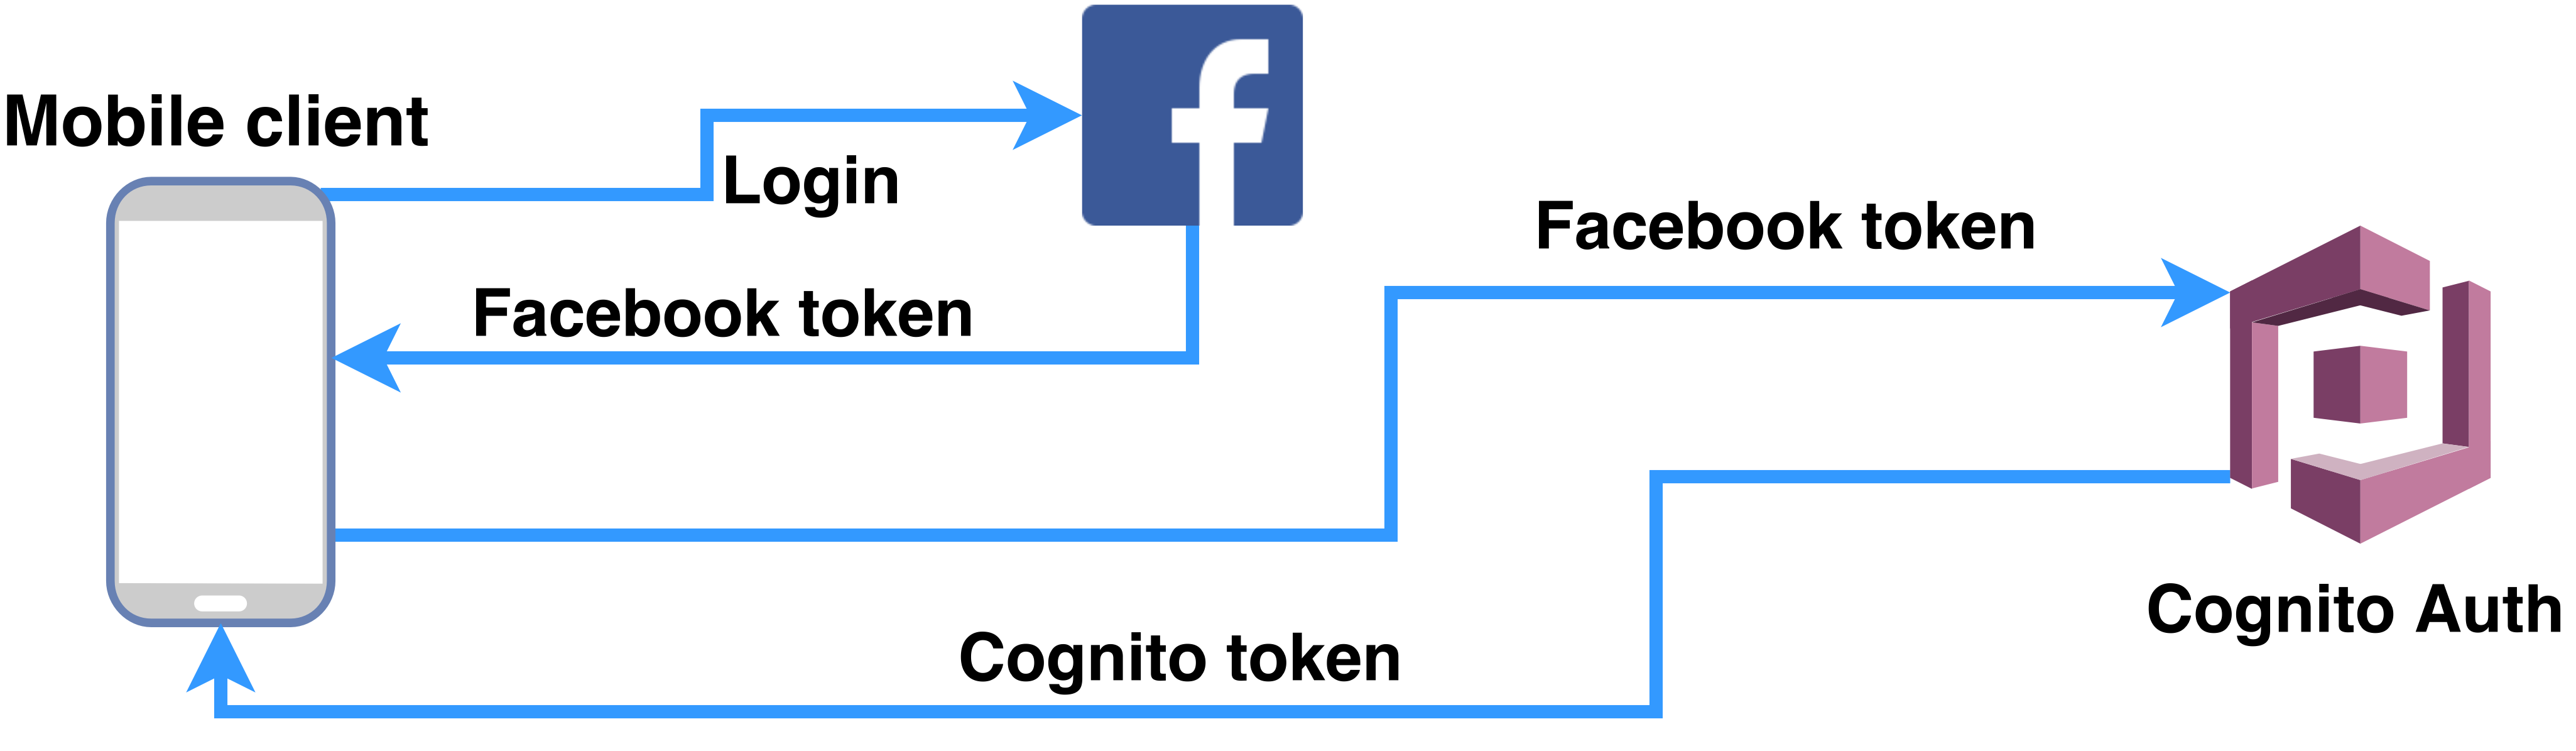
\includegraphics[scale=0.5]{../img/mobile_auth.png}}
\end{frame}


\begin{frame}
\frametitle{Container e load balancing}
\centerline{\includegraphics[scale=0.5]{../img/elastic.png}}
\end{frame}


\begin{frame}
\frametitle{Cache hit/miss}
\centerline{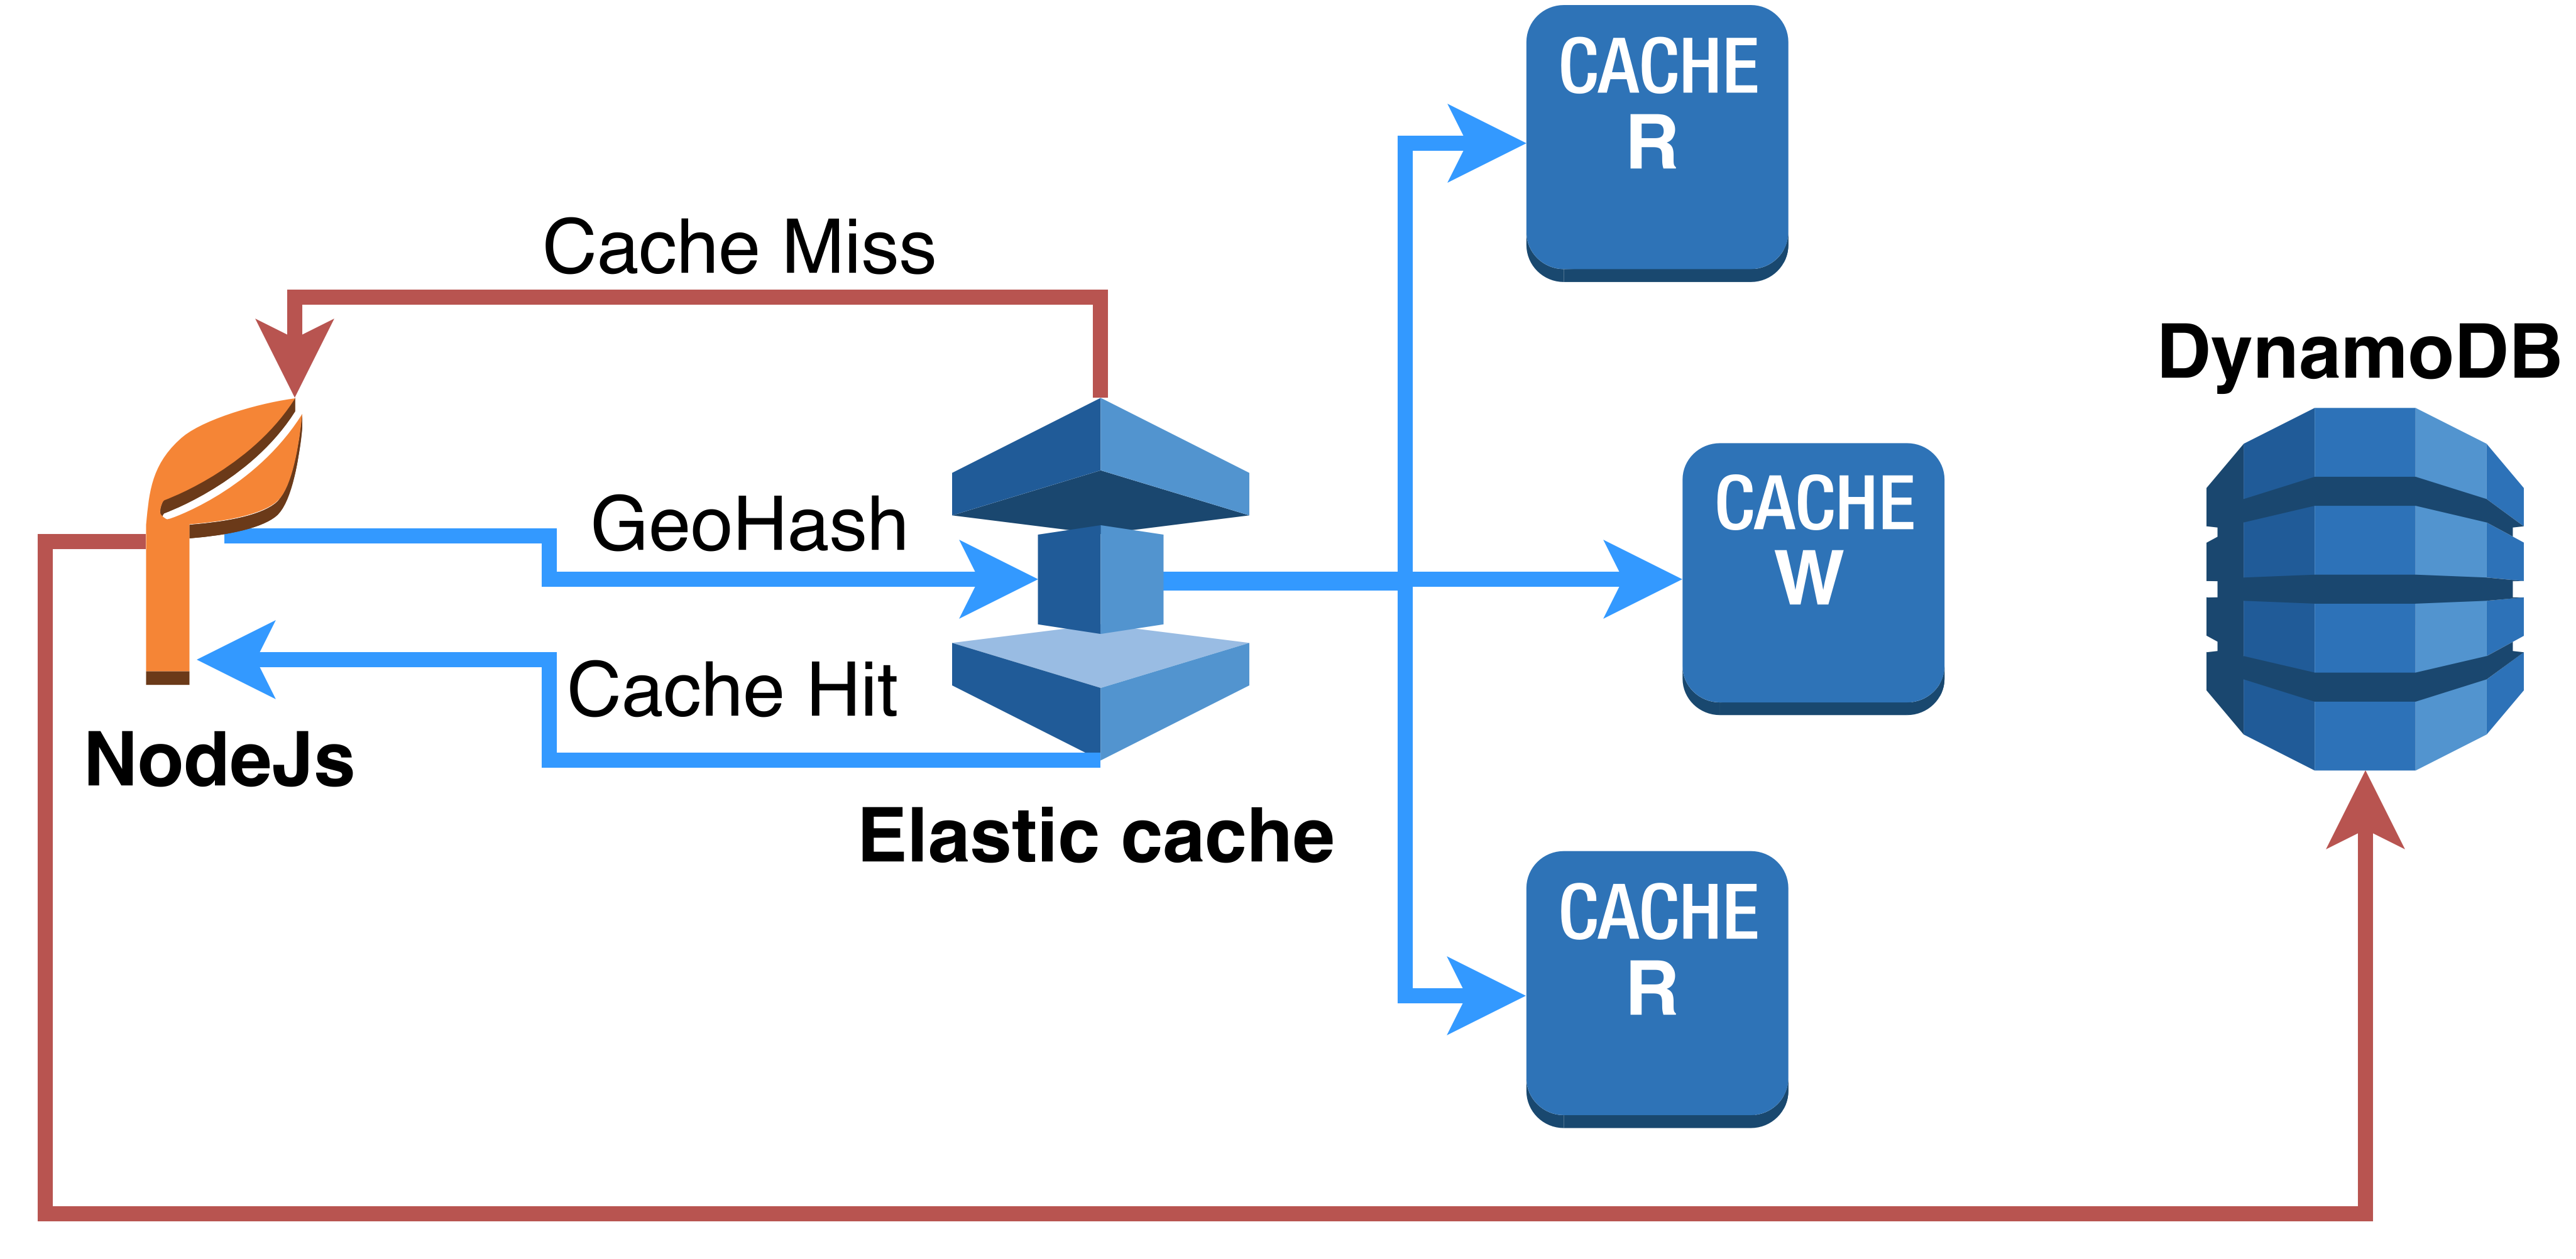
\includegraphics[scale=0.5]{../img/DataFetch.png}}
\end{frame}



\begin{frame}
\frametitle{Publish/Subscribe}
\centerline{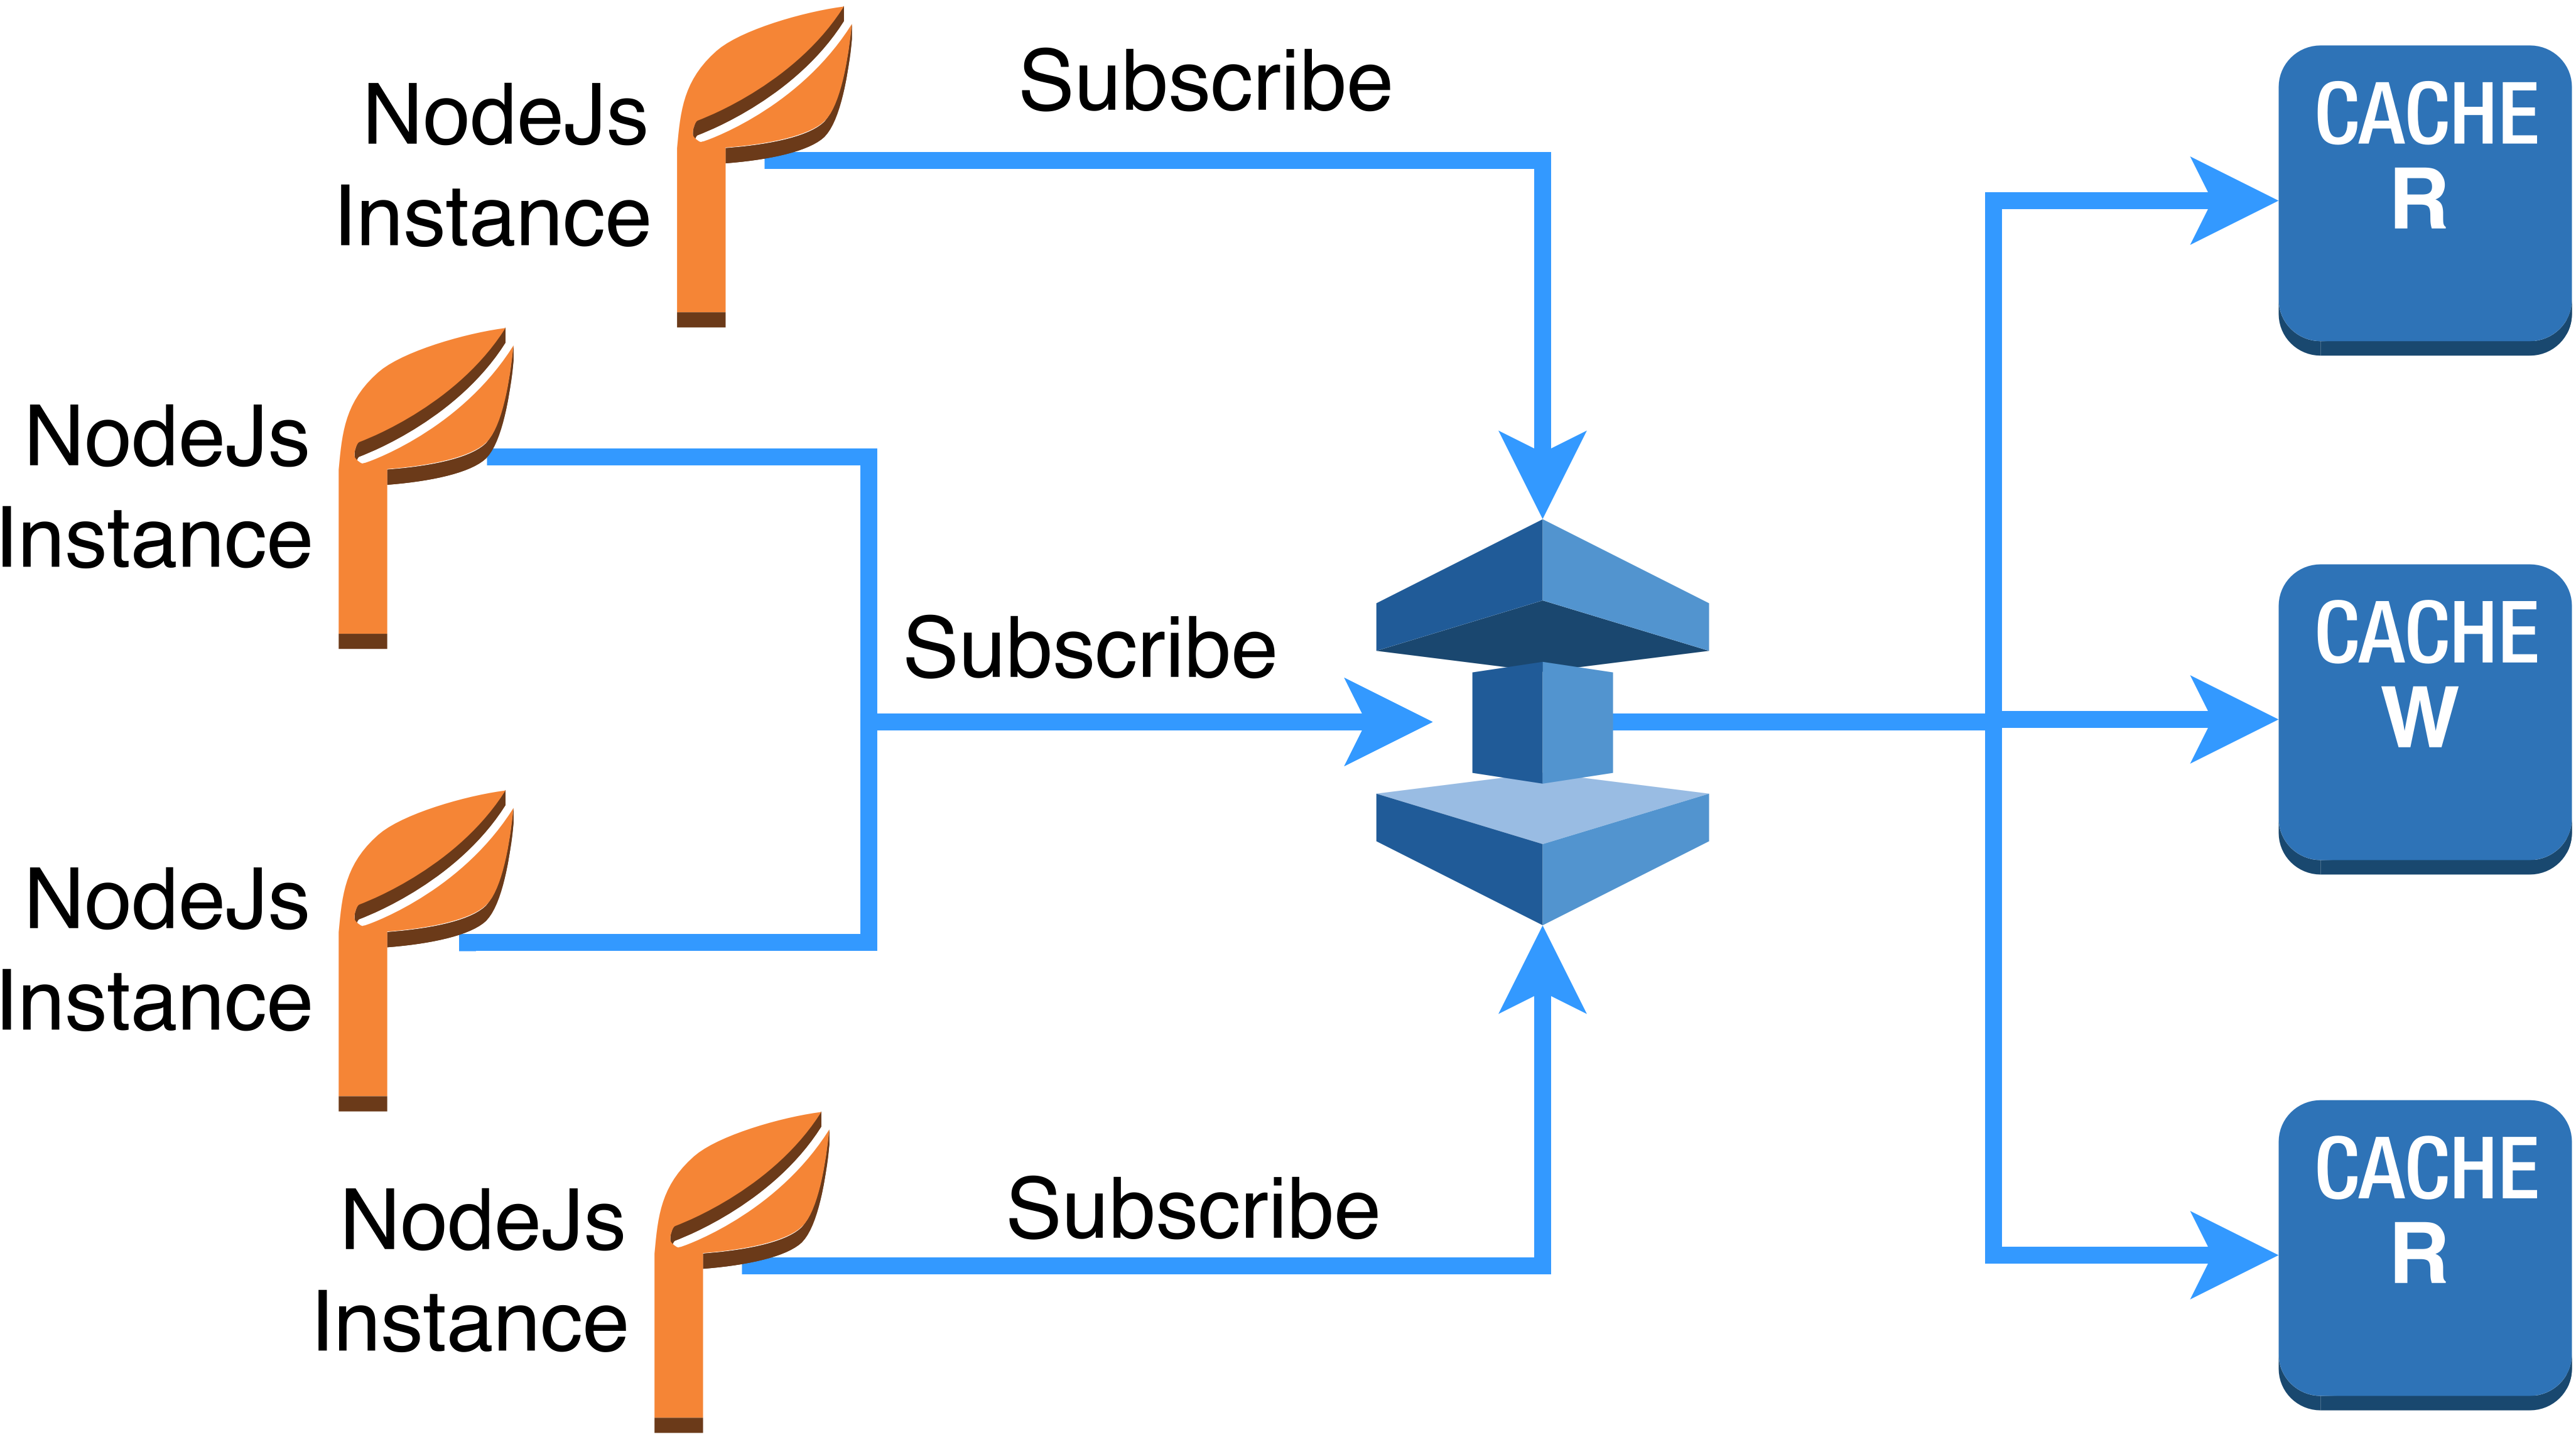
\includegraphics[scale=0.5]{../img/subscribe.png}}
\end{frame}

\begin{frame}
\frametitle{Websocket notification}
\centerline{\includegraphics[scale=0.5]{../img/updateps.png}}
\end{frame}





%SLIDE 5
\begin{frame}
\Huge{\centerline{The End}}
\end{frame}

%----------------------------------------------------------------------------------------

\end{document}
